\documentclass[a4paper,12pt]{article}

\usepackage{cmap}          % поиск в PDF
\usepackage{mathtext}         % русские буквы в формулах
\usepackage[T2A]{fontenc}      % кодировка
\usepackage[utf8]{inputenc}      % кодировка исходного текста
\usepackage[english,russian]{babel}  % локализация и переносы
\usepackage[left=2cm,right=2cm,top=2cm,bottom=2cm]{geometry}
\usepackage{amsfonts,amssymb,amsthm,mathtools} % AMS
\usepackage{amsmath}
\usepackage{icomma} % "Умная" запятая: $0,2$ --- число, $0, 2$
\usepackage{graphicx}
\usepackage{wrapfig} % картинка в тектсе
\usepackage{caption} % убирается номер у подписей caption*{}
\usepackage{csquotes} % цитаты
\usepackage{multirow} % для жестких таблиц
\usepackage{hhline}
\usepackage{indentfirst} % абзацный отступ после section
\usepackage{epigraph} % эпиграф
\usepackage{tikz}
\usepackage{pgfplots}
\usepackage[export]{adjustbox}
\usepackage{tabularx}
\usepackage{float}
\usepackage{longtable}
\begin{document}



\title{\textbf{Эффект Джоуля–Томсона. (2.1.6)}}
\author{Зайнуллин Амир}

\maketitle

\section{Аннотация}
    \textbf{Цели работы:} определение изменения температуры углекислого газа при протекании через малопроницаемую перегородку при разных начальных значениях давления и температуры.
    Вычисление по результатам опытов коэффициентов Ван-дер-Ваальса «a» и «b». \par
    \textbf{Оборудование:} трубка с пористой перегородкой; труба Дьюара; термостат; термометры; дифференциальная термопара; микровольтметр; балластный баллон; манометр.

\section{Теоретические сведения}

    \textbf{Эффектом Джоуля–Томсона} называется изменение температуры газа, медленно протекающего из области высокого в область низкого давления в условиях хорошей тепловой изоляции. 
    В разреженных газах, которые приближаются по своим свойствам к идеальному газу, при таком течении температура газа не меняется. Эффект Джоуля–Томсона демонстрирует отличие исследуемого газа от идеального. \par
    \textbf{Упрощения:} Макроскопическая скорость газа с обеих сторон трубки достаточно мала. Значит энтальпию газа можно считать постоянной величиной. \par 
    \medskip
    Уравнение состояния газа Ван-дер-Ваальса для одного моля:
    \begin{equation}
        (P + \dfrac{a}{V^2})(V - b) = RT
    \end{equation}

    Здесь a и b — коэффициенты Ван-дер-Ваальса, которые считаются постоянными. Формула (1) записана для одного моля газа, для $\nu$ молей вместо $V$ нужно использовать $\dfrac{V}{\nu}$
    
    \bigskip
    
    Используя упрощения можно получить формулу для коэффициента Джоуля-Томсона.
    \begin{equation}
    \mu_\text{д-т} = \frac{\Delta T}{\Delta P} \approx \frac{(2a/RT) - b}{C_P}
    \end{equation}

    Из формулы видно, что эффект Джоуля–Томсона для не очень плотного газа зависит от соотношения величин $ a $ и $ b $, которые оказывают противоположное влияние на знак эффекта. Если силы взаимодействия между молекулами велики, так что превалирует <<поправка на давление>>, то основную роль играет член, содержащий $ a $, и 

\[ \frac{\Delta T}{\Delta P} > 0, \]
т. е. газ при расширении охлаждается ($ \Delta T < 0 $, так как всегда $ \Delta P < 0 $). В обратном случае (малые $ a $)

\[ \frac{\Delta T}{\Delta P} < 0, \]
т. е. газ нагревается ($ \Delta T > 0 $, так как по-прежнему $ \Delta P < 0 $).

Этот результат нетрудно понять из энергетических соображений. Как мы уже знаем, у идеального газа эффект Джоуля–Томсона отсутствует. Идеальный газ отличается от реального тем, что в нем можно пренебречь потенциальной энергией взаимодействия молекул. Наличие этой энергии приводит к охлаждению или нагреванию реальных газов при расширении. При больших a велика энергия притяжения молекул. Это означает, что потенциальная энергия молекул при их сближении уменьшается, а при удалении -- при расширении газа -- возрастает. Возрастание потенциальной энергии молекул происходит за счет их кинетической энергии -- температура газа при расширении падает. Аналогичные рассуждения позволяют понять, почему расширяющийся газ нагревается при больших значениях $ b $.

Как следует из формулы, при температуре \[ T_i = \frac{2a}{Rb} \] коэффициент $ \mu_\text{д--т} $ обращается в нуль. По формулам связи параметров газа Ван-дер-Ваальса с критическими параметрами получаем: 

\begin{equation}
T_\text{инв} = \frac{27}{4} T_\text{кр}.
\end{equation}

При температуре $ T_\text{инв} $ эффект Джоуля–Томсона меняет знак: ниже температуры инверсии эффект положителен ($ \mu_\text{д--т} > 0 $, газ охлаждается), выше $ T_\text{инв} $ эффект отрицателен ($ \mu_\text{д--т} < 0 $, газ нагревается).

В данной лабораторной работе исследуется коэффициент дифференциального эффекта Джоуля–Томсона для углекислого газа. По экспериментальным результатам оценивается коэффициент теплового расширения, постоянные в уравнении Ван-дер-Ваальса и температура инверсии углекислого газа.

\section{Экспериментальная установка}

\begin{figure}[H]
    \centering
    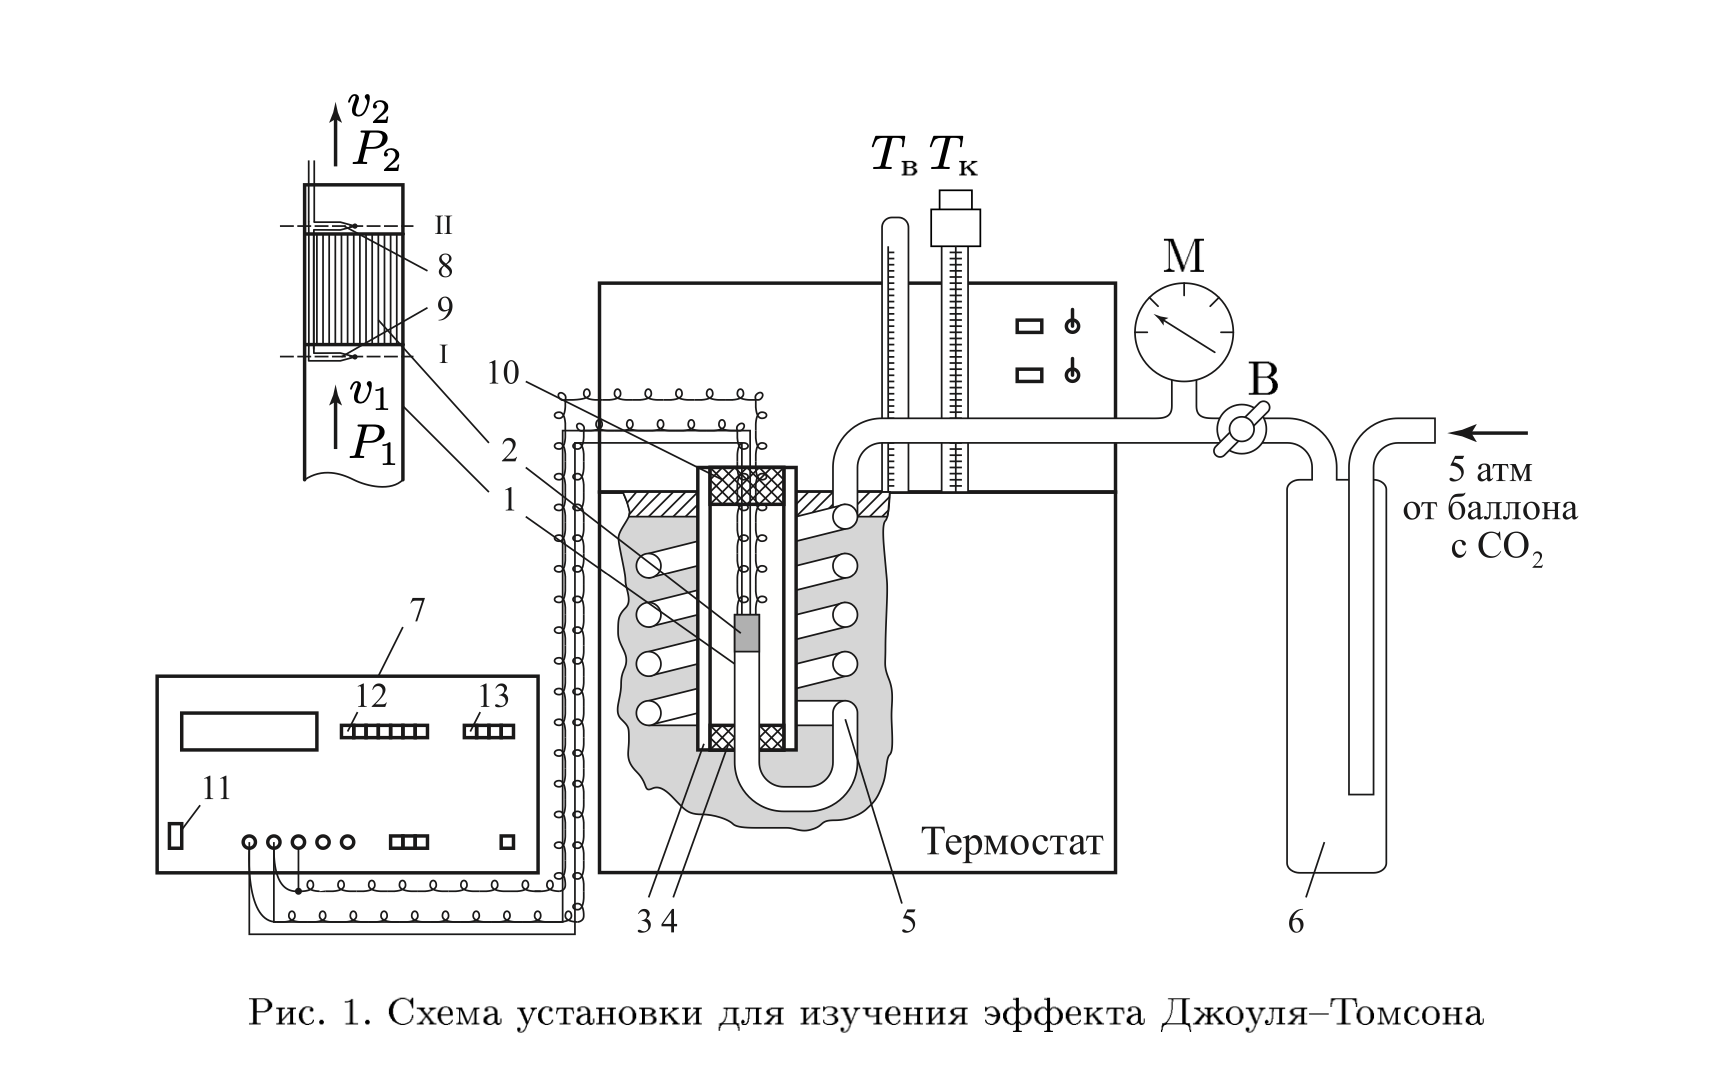
\includegraphics[width=0.83\textwidth]{7.png}
\end{figure}
На рисунке обозначены: трубка с пористой перегородкой (1), пористая перегородка (2), труба Дьюара (3), кольцо (4), змеевик (5), балластный баллон (6), вольтметр (7), верхний спай термопары (8), нижний спай термопары (9), пробка из пенопласта (10).

\begin{table}[!ht]
    \centering
    \begin{tabular}{|c|c|c|c|c|c|}
    \hline
    Температура, $^\circ C$ & 0-10 & 10-20 & 20-30 & 30-40 & 40-50 \\ \hline
    мкВ$/^\circ C$ & 38,9 & 39,8 & 40,7 & 41,6 & 42,5 \\ \hline
    \end{tabular}
    \caption {Зависимости приведённого напряжения от температуры}
\end{table}


\section{Результаты измерений и обработка данных}



Проведём измерение зависимости $ \Delta T $ от $ \Delta P $ для разных значений температур. Полученные значения заносим в таблицы. При записи полученных данных также учитываем, что чувствительность термопары зависит от температуры. При вычислении будем использовать следующую формулу: $ \Delta T = \frac{U}{\alpha}$.
\\ Погрешность $ \Delta T $ найдем по формуле: $ \sigma_{\Delta T} = \Delta T \frac{\sigma_U}{U_{ист}}$. Для нашего прибора $\sigma_U = 0,002$ мВ.
\\ Погрешность $ \Delta P$ находим зная класс точности манометра который равен 1. У манометра $P_{max} = 6 \text{ атм}$. Тогда $\sigma_p = 0,01 \cdot 6 = 0,06 \text{ атм}$.


\begin{table}[!ht]
    \centering
    \begin{tabular}{|c|c|c|c|c|c|c|}
    \hline
        $ \Delta P $, атм & $ \sigma_p $, атм & $ U $, мВ & $ U_{ист} $, мВ &$ \sigma_U $, мВ & $ \Delta T $, K & $ \sigma_{\Delta T} $, K \\ \hline
        4 & 0,06 & 0,124 & 0,122 & 0,002 & 3,00 & 0,05  \\ \hline
        3,5 & 0,06 & 0,104 & 0,102 & 0,002 & 2,51 & 0,05  \\ \hline
        3 & 0,06 & 0,084 & 0,082 & 0,002 & 2,01 & 0,05  \\ \hline
        2,5 & 0,06 & 0,064 & 0,062 & 0,002 & 1,52 & 0,05  \\ \hline
        2 & 0,06 & 0,044 & 0,044 & 0,002 & 1,08 & 0,05 \\ \hline
    \end{tabular}
    \caption{Экспериментальные данные для 21 $^\circ$C}
\end{table}

\begin{figure}[H]
    \centering
    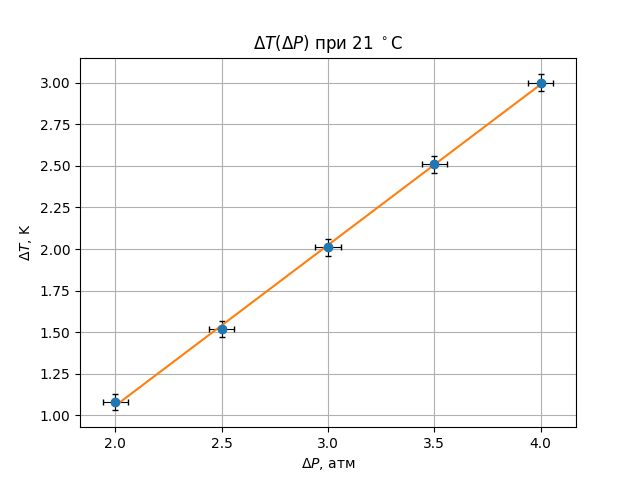
\includegraphics[width=0.79\textwidth]{1.png}
    \caption{График зависимости для 21 $^\circ$C}
\end{figure}

\begin{table}[!ht]
    \centering
    \begin{tabular}{|c|c|c|c|c|c|c|}
    \hline
        $ \Delta P $, атм & $ \sigma_p $, атм & $ U $, мВ & $ U_{ист} $, мВ &$ \sigma_U $, мВ & $ \Delta T $, K & $ \sigma_{\Delta T} $, K \\ \hline
        4 & 0,06 & 0,118 & 0,116 & 0,002 & 2,85 & 0,05  \\ \hline
        3,5 & 0,06 & 0,100 & 0,098 & 0,002 & 2,41 & 0,05  \\ \hline
        3 & 0,06 & 0,083 & 0,081 & 0,002 & 1,99 & 0,05  \\ \hline
        2,5 & 0,06 & 0,066 & 0,064 & 0,002 & 1,57 & 0,05  \\ \hline
        2 & 0,06 & 0,052 & 0,050 & 0,002 & 1,23 & 0,05 \\ \hline
    \end{tabular}
    \caption{Экспериментальные данные для 25 $^\circ$C}
\end{table}

\begin{figure}[H]
    \centering
    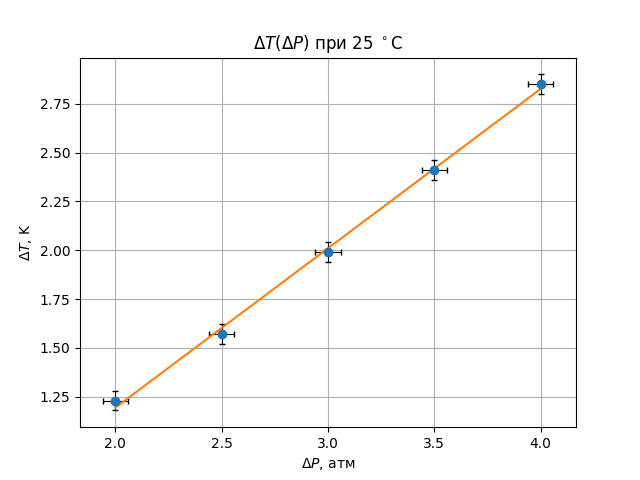
\includegraphics[width=0.85\textwidth]{2.png}
    \caption{График зависимости для 25 $^\circ$C}
\end{figure}

\begin{table}[!ht]
    \centering
    \begin{tabular}{|c|c|c|c|c|c|c|}
    \hline
        $ \Delta P $, атм & $ \sigma_p $, атм & $ U $, мВ & $ U_{ист} $, мВ &$ \sigma_U $, мВ & $ \Delta T $, K & $ \sigma_{\Delta T} $, K \\ \hline
        4 & 0,06 & 0,117 & 0,113 & 0,002 & 2,72 & 0,05  \\ \hline
        3,5 & 0,06 & 0,104 & 0,100 & 0,002 & 2,40 & 0,05  \\ \hline
        3 & 0,06 & 0,087 & 0,083 & 0,002 & 2,00 & 0,05  \\ \hline
        2,5 & 0,06 & 0,064 & 0,060 & 0,002 & 1,44 & 0,05  \\ \hline
        2 & 0,06 & 0,048 & 0,044 & 0,002 & 1,06 & 0,05 \\ \hline
    \end{tabular}
    \caption{Экспериментальные данные для 35 $^\circ$C}
\end{table}

\begin{figure}[!ht]
    \centering
    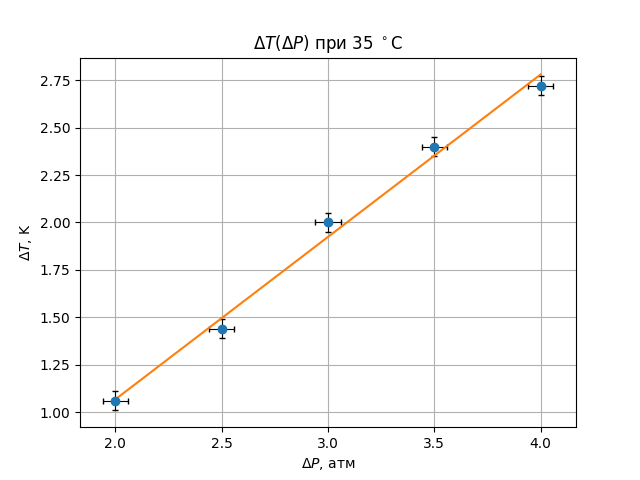
\includegraphics[width=0.85\textwidth]{3.png}
    \caption{График зависимости для 35 $^\circ$C}
\end{figure}

\begin{table}[!ht]
    \centering
    \begin{tabular}{|c|c|c|c|c|c|c|}
    \hline
        $ \Delta P $, атм & $ \sigma_p $, атм & $ U $, мВ & $ U_{ист} $, мВ &$ \sigma_U $, мВ & $ \Delta T $, K & $ \sigma_{\Delta T} $, K \\ \hline
        4 & 0,06 & 0,112 & 0,108 & 0,002 & 2,54  & 0,05  \\ \hline
        3,5 & 0,06 & 0,095 & 0,091 & 0,002 & 2,14  & 0,05  \\ \hline
        3 & 0,06 & 0,078 & 0,074 & 0,002 & 1,74  & 0,05  \\ \hline
        2,5 & 0,06 & 0,061 & 0,057 & 0,002 & 1,34  & 0,05  \\ \hline
        2 & 0,06 & 0,045 & 0,041 & 0,002 & 0,96 & 0,05 \\ \hline
    \end{tabular}
    \caption{Экспериментальные данные для 45 $^\circ$C}
\end{table}

\begin{figure}[H]
    \centering
    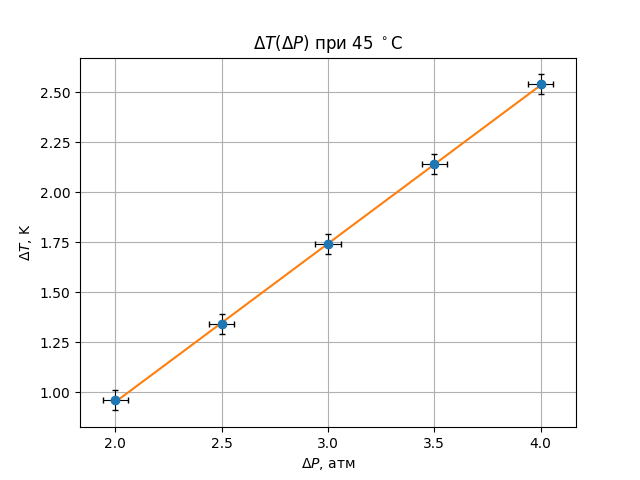
\includegraphics[width=0.85\textwidth]{4.png}
    \caption{График зависимости для 45 $^\circ$C}
\end{figure}

\begin{table}[H]
    \centering
    \begin{tabular}{|c|c|c|c|c|c|c|}
    \hline
        $ \Delta P $, атм & $ \sigma_p $, атм & $ U $, мВ & $ U_{ист} $, мВ &$ \sigma_U $, мВ & $ \Delta T $, K & $ \sigma_{\Delta T} $, K \\ \hline
        4 & 0,06 & 0,090 & 0,086 & 0,002 & 1,99  & 0,05  \\ \hline
        3,5 & 0,06 & 0,075 & 0,071 & 0,002 & 1,64  & 0,05  \\ \hline
        3 & 0,06 & 0,062 & 0,058 & 0,002 & 1,34  & 0,05  \\ \hline
        2,5 & 0,06 & 0,050 & 0,046 & 0,002 & 1,06  & 0,05  \\ \hline
        2 & 0,06 & 0,040 & 0,036 & 0,002 & 0,83 & 0,05 \\ \hline
    \end{tabular}
    \caption{Экспериментальные данные для 55 $^\circ$C}
\end{table}

\begin{figure}[H]
    \centering
    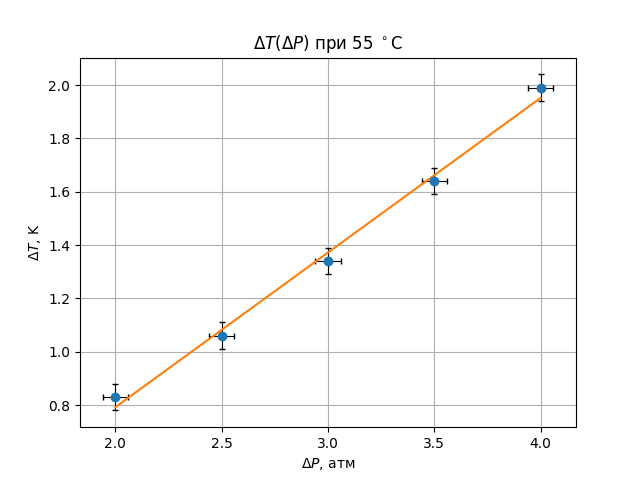
\includegraphics[width=0.85\textwidth]{5.png}
    \caption{График зависимости для 55 $^\circ$C}
\end{figure}

Чтобы определить коэффициент Джоуля-Томсона, посчитаем коэффициент наклона графика $\Delta T$ от $\Delta P$. На рисунках изображены графики зависимостей.

Вычислим $ \mu_\text{д--т} = \frac{dT}{dP} $, используя МНК:

\[ \mu_\text{д--т} = \frac{\langle \Delta P \Delta T \rangle - \langle \Delta P \rangle \langle \Delta T \rangle}{\langle \Delta P^2 \rangle - \langle \Delta P \rangle ^2}.\]

Случайную погрешность определения этого коэффициента вычислим по следующей~формуле:

\[ \sigma_{случ} = \frac{1}{\sqrt{n}} \cdot \sqrt{\frac{\langle \Delta T^2 \rangle - \langle \Delta T \rangle^2}{\langle \Delta P^2 \rangle - \langle \Delta P \rangle ^2} - \mu_\text{д--т}^2}\] где  $ n $  -- колличество измерений.

Систематическую ошибку будем считать по формуле 
\[ \sigma_\text{сист} = {\mu_\text{д--т}}\sqrt{\varepsilon^2_{\Delta P}+\varepsilon^2_{\Delta T}}.\]
Где относительная погрешность будет считаться для среднего значения $P = 3\text{ атм}$ \\
Полная погрешность равна 
\[ \sigma = \sqrt{\sigma_{случ}^2 + \sigma_\text{сист}^2} \]
\par Полученные результаты заносим в таблицу.

\begin{table}[!ht]
    \centering
    \begin{tabular}{|c|c|c|c|c|c|c|}
    \hline
        $t\text{, }^\circ$C & $T$, К & $\frac{1}{T} \cdot 10^3 \text{, } \frac{1}{\text{К}} \cdot 10^3$ & $\mu_\text{д--т} \text{, } \frac{\text{К}}{\text{атм}}$ & $\sigma_{случ} \text{, } \frac{\text{К}}{\text{атм}}$ & $\sigma_{сист} \text{, } \frac{\text{К}}{\text{атм}}$ & $\sigma \text{, } \frac{\text{К}}{\text{атм}}$ \\ \hline
        21 & 294 & 3,40 & 0,966 & 0,009 & 0,031 & 0,032  \\ \hline
        25 & 298 & 3,36 & 0,816 & 0,012 & 0,026 & 0,029  \\ \hline
        35 & 308 & 3,25 & 0,856 & 0,022 & 0,027 & 0,035  \\ \hline
        45 & 318 & 3,14 & 0,792 & 0,003 & 0,028 & 0,028  \\ \hline
        55 & 328 & 3,05 & 0,58 & 0,014 & 0,025 & 0,028 \\ \hline
    \end{tabular}
\end{table}

\subsection*{Определение постоянных $a$, $b$ и $T_i$ для углекислого газа (11 пункт)}
Из следующей формулы следует, что график $\mu_\text{д--т} \text{ от } \frac{1}{T}$ должен быть линейным. 
    \[ \mu_\text{д-т} = \frac{\Delta T}{\Delta P} \approx \frac{(2a/RT) - b}{C_P} \]
Построим его, и найдем коэффициенты $a \text{ и } b$
    
\begin{figure}[H]
    \centering
    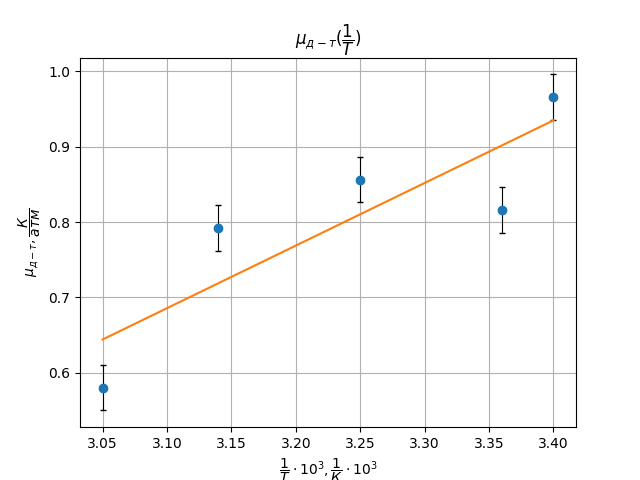
\includegraphics[width=0.85\textwidth]{6.png}
    \caption{График зависимости $\mu_\text{д-т}$ от $\dfrac{1}{T}$}
\end{figure}
\[ k_{накл} = 831 \cdot \dfrac{K^2}{атм} \quad \varepsilon_{случ} = 0,08 \quad \varepsilon_{сист} = 0,04 \quad \varepsilon = \sqrt{\varepsilon_{случ}^2 + \varepsilon_{сист}^2} = 0,1\]
\[ a = \dfrac{k_{накл}RC_p}{2} \]
\[ a = (1,38 \pm 0,14) \dfrac{Н \cdot м^4}{\text{моль}^2} \]

\[ -\dfrac{b}{C_{p}} = -1,89 \frac{\text{К}}{\text{атм}} \quad \sigma = \sigma_{a} \sqrt{\langle \dfrac{1}{T^2} \rangle - \langle \dfrac{1}{T} \rangle^2} \]
\[ {b} = (756 \pm 99) \dfrac{\text{см}^3}{\text{моль}^2}  \]

\subsection*{Вычисление температуры инверсии}
Из теоретической сведений выше $T_i = \frac{2a}{Rb}$. По найденным параметрам $a$ и $b$ вычислим. 
\[ T_i = (440 \pm 101) \text{ K}\]

\section{Вывод (12 пункт)} 

В данной лабораторной работе мы исследовали Эффект Джоуля-Томсона. Из зависимости изменения температуры углекислого газа при протекании через малопроницаемую перегородку 
при разных начальных значениях давления и температуры мы находили коэффициент Джоуля Томсона для разных температурах аппроксимируя график  зависимости $\Delta T(\Delta P)$.
\\ Построив график зависимости $\mu_\text{д-т}$ от $\dfrac{1}{T}$ нашли коэфициенты газа Ван-Дер-Ваальса. Для углекислого газа табличные данные равны $a = 0,364 \dfrac{Н \cdot м^4}{\text{моль}^2}$ и 
${b} = 42,6 \dfrac{\text{см}^3}{\text{моль}^2}$. Видно, что полученные данные сильно расходятся с табличными. Это может быть связано с тем, что наши упрощения, которые мы использовали чтобы вывести формулу коэффициента Джоуля-Томсона не выполняются. 
Возможно также приближения реального газа формулой Ван-дер-Ваальса не совсем точно. Расхождение с табличным значением $T_i = 2053 \text{ K}$ возможно вызвано теми же проблемами. 


\end{document}